\documentclass{cys}

\usepackage[utf8]{inputenc}

%\usepackage[english]{babel}
%\usepackage[spanish,mexico,es-tabla]{babel}
\usepackage[russian,english]{babel}  % If you use other languages, use Babel package.

\usepackage{moreverb}
%\usepackage[breaklinks,colorlinks,bookmarksopen,bookmarksnumbered,linkcolor=ICSTblue,citecolor=blue,urlcolor=ICSTblue]{hyperref}
\usepackage{amsmath,amssymb,amsfonts}
\usepackage{algorithmic}
\usepackage[ruled,linesnumbered]{algorithm2e}
\usepackage{textcomp}
\usepackage{xcolor}
\usepackage{breakurl}
\usepackage{doi}
\usepackage{cancel}
\usepackage{amsmath}
\usepackage{array}
\usepackage{setspace}
\usepackage{tabu}                      % only used for the table example
\usepackage{booktabs}                  % only used for the table example
\usepackage{eqparbox}
\usepackage{graphicx}
\usepackage{textcomp}
\usepackage{xcolor}
\usepackage{subcaption}
\usepackage{caption}
\usepackage{multicol} % for multi-column support
\usepackage{enumitem}
\usepackage{graphicx}
\usepackage{xcolor}
\usepackage{epstopdf} % Avoid using plain Latex, use PDFLATEX
\usepackage{amsmath} % For align environment
\usepackage{booktabs}
\addto\captionsenglish{%
  \renewcommand{\figurename}{Fig.}%
  \renewcommand{\abstractname}{Abstract.} 
%  \renewcommand{\keywordsname}{Keywords: } 
}

\addto\captionsspanish{%
  \renewcommand{\figurename}{Fig.}%
  \renewcommand{\abstractname}{Resumen.} 
%  \renewcommand{\keywordsname}{Palabras clave: } 
}


\title{L-GRU: Building a Hybrid Model to Improve Stock Price Prediction}

\author{Tran Dinh Dang$^1$, Sittixay Chounlamany$^1$, Nguyen Quoc Dung$^1$, Le Mai Nam$^2$, \\Le Thi Huyen Trang$^2$, Nguyen Viet Hung$^{3,*}$}

\affil{ 
$^1$ Faculty of Information Technology, Ha Tinh University, Hatinh, Vietnam            
\authorcr \authorcr
$^2$ Faculty of Information Technology, East Asia University of Technology, Bacninh, Vietnam            
\authorcr \authorcr
$^3$ International Training and Cooperation Institute, East Asia University of Technology, Bacninh, Vietnam            
\authorcr  \authorcr
\{11231502003, 11231502023\}@hu.edu.vn, dung.nguyenquoc@htu.edu.vn, \\\{namlm, tranglth, hungnv\}@eaut.edu.vn
\authorcr \authorcr
}


\begin{document}

\maketitle

\renewcommand{\tablename}{Table}

\begin{abstract}
The rapid advancement of artificial intelligence (AI) has transformed financial forecasting by enabling the analysis of large-scale time series data and uncovering complex market patterns. However, a fundamental trade-off persists: Long Short-Term Memory (LSTM) networks offer strong long-term memory retention but are computationally costly, while Gated Recurrent Units (GRUs) provide efficiency at the expense of long-range fidelity. To address this gap, we propose \textbf{L-GRU}, a novel recurrent cell architecture that preserves the dedicated cell state of LSTM while adopting the streamlined update mechanism of GRU, further enhanced with a Relevance Gate, peephole connections, and layer normalization. Evaluated on Tesla Inc.’s stock price data from 2015 to 2024, L-GRU consistently outperforms established baselines, including LSTM, GRU, Transformer, and hybrid models, achieving a coefficient of determination ($R^2$) of 0.9688 and reducing mean squared error by more than 50\% compared to the best baseline. These results establish L-GRU as a new benchmark for financial time series forecasting, offering both improved predictive accuracy and practical value for data-driven investment decision-making.

%In recent years, advancements in information technology have significantly influenced the financial markets, prompting investors to seek innovative approaches for gaining competitive advantages and formulating effective strategies. Decision-making has become increasingly crucial, particularly with the rapid development of artificial intelligence (AI), which has enhanced the ability to analyze vast amounts of data, identify potential trends, and forecast future market behaviors. This study introduces a hybrid methodology that integrates Long Short-Term Memory (LSTM) and Gated Recurrent Unit (GRU) models (we called L-GRU) to leverage the strengths of both techniques, achieving improved forecasting accuracy compared to existing models. Experimental results demonstrate that the proposed model achieves up to a \textcolor{red}{....\%} improvement in prediction accuracy over benchmark models. This enhanced forecasting capability provides investors with deeper insights into market dynamics, enabling more informed and strategic decision-making.
\end{abstract}

\begin{keywords} 
Information Technology,  Financial Markets, Artificial Intelligence, Long Short-Term Memory, Gated Recurrent Unit, Forecasting Accuracy.
\end{keywords} 

%%%%%%%%%%%%%%%% THIS SECTION ONLY if your paper is in Spanish:

% \othertitle{Title in Spanish, only if your paper is in Spansih}

% \begin{abstract}
% Resumen en español ...
% \end{abstract}

% \begin{keywords} 
% Palabra1, palabrs2, palabra3.
% \end{keywords} 

%%%%%%%%%%%%%%%%

\section{Introduction}

The stock market is widely recognized as a cornerstone of the global economy, not only serving as a platform for capital mobilization but also acting as a critical barometer of economic health \cite{xiao2024comparative}. Its influence extends to investors, policymakers, and the general public, making accurate prediction of stock price dynamics an issue of both theoretical and practical importance. Within this context, the Efficient Market Hypothesis (EMH) provides a well-established theoretical foundation, suggesting that in an ideal market, stock prices fully and instantaneously reflect all available information \cite{genot2024predictive, ronkko2024adaptive, ehiedu2022efficient, malkiel2011efficient, lachaari2021capital}.

In practice, however, financial markets deviate significantly from this idealized efficiency. Stock prices are influenced by a wide range of nonlinear and interdependent factors, including investor psychology, market sentiment, macroeconomic conditions, and geopolitical shocks \cite{akinrinola2024predicting, satishbhai2025stock}. These dynamics create strong non-stationarity, high volatility, and complex temporal dependencies that traditional econometric models are unable to capture effectively. As a result, more advanced computational techniques are required to address the inherent unpredictability of financial time series.

In recent years, deep learning—particularly Recurrent Neural Networks (RNNs)—has demonstrated strong potential for modeling sequential data such as stock prices. Among these, Long Short-Term Memory (LSTM) networks and Gated Recurrent Units (GRU) have emerged as leading architectures. LSTM excels at modeling long-term dependencies through its explicit memory cell, while GRU offers faster training and fewer parameters, making it computationally efficient. However, each architecture faces trade-offs: LSTM is often computationally heavy, whereas GRU, though lightweight, may lose fidelity in capturing long-range patterns. Hybrid approaches that attempt to combine LSTM and GRU have therefore emerged as promising solutions \cite{alomar2024rnns, bhavani2022comparative, karim2022stock, chavhan2024deep}. In addition, recent studies have also explored the application of deep learning to sequential prediction tasks in domains such as 360-degree video streaming, where LSTM and GRU have been used successfully for accurate viewport estimation \cite{hung2025building, nguyen2022accurate, hung2025heverl}. While these works primarily address challenges in immersive media, they highlight the effectiveness of recurrent architectures in modeling complex, nonstationary sequences—an ability that is equally critical for financial time series forecasting. Motivated by these insights, this study introduces L-GRU, a redesigned recurrent cell specifically designed to improve stock price prediction.

Despite these efforts, most existing hybrids rely on architectural stacking or ensembling rather than rethinking the core recurrent cell. As such, they fail to fully reconcile the fundamental trade-off between the memory fidelity of LSTM and the efficiency of GRU. This observation motivates our central research question: Can a new recurrent unit be designed to simultaneously preserve the explicit long-term memory of LSTM while operating with the streamlined gating mechanism of GRU?

To answer this question, we propose L-GRU, a novel recurrent cell architecture specifically tailored for financial time series forecasting. Unlike traditional hybrid approaches, L-GRU is not a simple combination but a redesigned recurrent unit. It retains the dedicated memory cell of LSTM, adopts a GRU-inspired update gate to simplify memory operations, and introduces a new Relevance Gate to filter irrelevant past information. Furthermore, architectural enhancements such as peephole connections, decoupled weight matrices, and layer normalization improve the model’s contextual awareness, stability, and training efficiency in Figure \ref{fig:placeholder}.

\begin{figure}
    \centering
    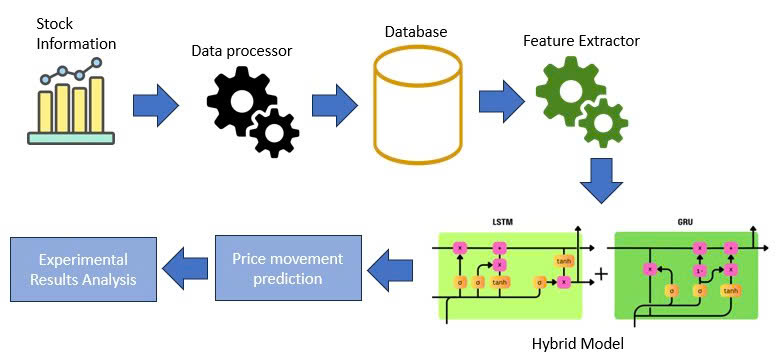
\includegraphics[width=\linewidth]{Figure/sysytem.PNG}
    \caption{Architecture system}
    \label{fig:placeholder}
\end{figure}

The contributions of this study are summarized as follows:
\begin{itemize}
    \item We propose L-GRU, a novel recurrent cell that integrates the strengths of LSTM and GRU while addressing their individual weaknesses.
    \item We introduce the Relevance Gate and other architectural refinements to enhance learning dynamics and prediction robustness.
    \item We provide a comprehensive experimental evaluation on real-world stock price data (Tesla Inc., TSLA), demonstrating that L-GRU significantly outperforms baseline models (LSTM, GRU, Transformer, and hybrid architectures) across multiple metrics.
    \item We establish L-GRU as a new benchmark for financial time series forecasting, offering both theoretical contributions and practical implications for investors and analysts.
\end{itemize}

The remainder of this paper is organized as follows. Section~\ref{sec:related_work} reviews related research on time series forecasting models. Section~\ref{sec:problem_formulation} details the proposed L-GRU methodology. Section~\ref{sec:evaluation} presents the experimental setup and evaluation results. Finally, Section~\ref{sec:conclusion} concludes the paper with key findings, limitations, and directions for future work.



\section{Related Work}\label{sec:related_work}

Stock price forecasting has long been a central theme in financial research due to the high volatility, nonlinearity, and non-stationarity of financial time series \cite{refenes1994stock}. Over the past decades, forecasting methods have evolved through three main stages: traditional econometric models, classical machine learning approaches, and modern deep learning architectures. This section reviews these developments, highlighting their strengths and limitations, and identifies the research gap that motivates the design of the proposed L-GRU model.

\subsection{Traditional Statistical and Econometric Models}
The origins of financial forecasting lie in statistical models such as the Autoregressive Integrated Moving Average (ARIMA) model \cite{box2015time}. ARIMA assumes that future values of a series can be expressed as a linear function of past values and forecast errors. While interpretable and parsimonious, ARIMA is fundamentally constrained by its linear assumption, making it ill-suited for the complex, nonlinear dynamics of financial markets \cite{makridakis2000m3}.

On the other hand, to capture volatility clustering a well-documented stylized fact in financial returns, the Generalized Autoregressive Conditional Heteroskedasticity (GARCH) family was introduced \cite{bollerslev1986generalized, rachev2011financial}. Extensions such as EGARCH and GJR-GARCH provide powerful tools for modeling conditional variance and remain indispensable in risk management and derivatives pricing \cite{engle1982autoregressive}. However, these models primarily forecast volatility rather than directional price movements, limiting their utility for trading strategies. Overall, statistical models lack the structural capacity to incorporate exogenous variables and to capture deep nonlinear patterns.

\subsection{Classical Machine Learning Methods}
The late 20th century witnessed a paradigm shift with the rise of machine learning. Support Vector Machines (SVMs), particularly in regression form (SVR), leveraged kernel methods to model nonlinear relationships in financial data \cite{cortes1995support}. While SVMs often outperform linear models in predicting stock movement \cite{huang2005forecasting}, they are computationally expensive for large-scale datasets and highly sensitive to kernel selection and hyperparameters.

Ensemble methods, such as Random Forests (RF) \cite{breiman2001random}, provided robustness against overfitting and offered feature importance scores for interpretability \cite{kumar2016random}. However, tree-based models are inherently non-sequential; they rely on handcrafted lag features and cannot naturally capture long-term temporal dependencies. Thus, while effective in static classification tasks, their capacity for sequential forecasting remains limited.


\subsection{Deep Learning Models for Sequential Data}
The advent of deep learning revolutionized financial time series analysis by enabling models that learn hierarchical feature representations directly from raw sequential data.

Recurrent Neural Networks (RNNs) introduced memory through recurrent connections, but their training was hindered by vanishing and exploding gradients \cite{bengio1994learning}.

Long Short-Term Memory (LSTM) networks overcame this limitation by introducing a dedicated cell state regulated by input, forget, and output gates \cite{hochreiter1997long}. This design allowed selective retention of long-term dependencies and established LSTM as a dominant baseline in stock forecasting \cite{fischer2018deep, moghar2020stock}.

Gated Recurrent Units (GRUs) streamlined the LSTM by merging the input and forget gates into a single update gate and combining the cell and hidden states \cite{cho2014learning}. This reduced parameter count improves efficiency and mitigates overfitting, especially on smaller datasets \cite{chung2014empirical}. Comparative studies \cite{xiao2024comparative, bhavani2022comparative, nguyen2022accurate} often show that LSTM and GRU perform competitively, with LSTM excelling in long-term memory preservation while GRU offers faster training.

Building on these foundations, hybrid and novel architectures have emerged. For example, CNN-LSTM models use convolutional layers for local feature extraction before LSTM modeling \cite{hoseinzade2019cnn}, while Transformer architectures leverage self-attention to capture long-range dependencies \cite{vaswani2017attention}. Although Transformers achieve state-of-the-art performance in many sequence tasks, their quadratic computational cost and lack of inductive bias for sequentiality can be inefficient for financial data.

\section{Proposed Method}\label{sec:problem_formulation}
This section details the proposed methodology, focusing on the architecture, mathematical foundations, and implementation workflow of the L-GRU (Long-term Gated Recurrent Unit) model. It is a hybrid recurrent neural network architecture developed to address the specific challenges of financial time-series forecasting. The section is organized as follows: first, we present an overview of the architecture and the rationale for integrating components from LSTM and GRU. Next, we provide a detailed derivation of the L-GRU cell’s mathematical formulation, tracing its development from the initial concept to the finalized model. We then describe the comprehensive experimental protocol, including data preprocessing steps and training strategies. Finally, we analyze the theoretical advantages of L-GRU relative to other baseline models.


\subsection{Architectural Overview and Theoretical Foundations}
The financial market is a complex, non-linear, and ever-evolving system in which asset prices are influenced by a multitude of factors, ranging from macroeconomic indicators to crowd psychology and unexpected events \cite{akinrinola2024predicting}. Time series data from this market inherently exhibit characteristics such as high volatility, non-stationarity, and the presence of intricate correlations that persist across multiple time horizons \cite{refenes1994stock}. These features present significant challenges for traditional forecasting models, which often rely on assumptions of linearity and data stability \cite{makridakis2000m3}.

Against this backdrop, deep learning models—particularly Recurrent Neural Networks (RNNs)—have emerged as powerful tools. Two advanced RNN architectures, Long Short-Term Memory (LSTM) and Gated Recurrent Unit (GRU), have demonstrated outstanding effectiveness. LSTM, introduced by Hochreiter and Schmidhuber (1997), excels at capturing long-term dependencies through a specialized memory structure known as the cell state, which functions like an “information conveyor belt” safeguarded and regulated by three gates (forget gate, input gate, and output gate) \cite{hochreiter1997long}. However, this complexity comes with high computational costs and a large number of parameters. In contrast, GRU, proposed by Cho ettal. (2014), is a more streamlined variant that merges the cell state and hidden state, while reducing the number of gates to two (reset gate and update gate) \cite{cho2014learning}. This simplification enables faster training and can help reduce the risk of overfitting on small datasets, though the merging of states may diminish the nuanced control over memory compared to LSTM \cite{chung2014empirical}.

From the above analysis, we pose a central research question: “Is it possible to design a new hybrid architecture that both inherits the powerful and distinct long-term memory mechanism of LSTM and operates it through the streamlined and efficient gating system of GRU?

\textcolor{red}{Đoạn này cần thiết kế một cái hình chi tiết về cấu trúc của mình đề xuất} The proposed L-GRU model is precisely our answer to this question. Our core hypothesis is that, by retaining the independent cell state (Ct) of LSTM while replacing the input/forget gate pair with a single update gate inspired by GRU, we can achieve a more optimal balance between long-term memory retention and computational efficiency. As illustrated in the overall architecture Figure \ref{fig:placeholder} Architecture system, L-GRU functions as the predictive core, integrated into a standardized machine learning workflow encompassing data collection, preprocessing, model training, and result analysis.


\subsection{Mathematical Formula of the L-GRU Model}
The design of the L-GRU model is the outcome of a systematic research process, involving the hybridization of foundational ideas followed by the integration of architectural enhancements to boost performance.

\begin{enumerate}
  \item \textbf{Foundational Hybridization Concept}

  This process begins with a detailed deconstruction of LSTM and GRU core components to identify opportunities for beneficial integration. The primary objective is to preserve the long-term memory capacity associated with the LSTM cell state while simplifying the gating structure to improve computational efficiency.
\end{enumerate}
  \begin{itemize}
    \item \textbf{Enhancing New Information Generation with the ``Relevance Gate'' (\(r_t\)):}

  In a standard LSTM, the candidate cell state \(\tilde{C}_t\)---representing potential new information---is generated directly from the previous hidden state \(h_{t-1}\) and the current input \(x_t\). However, \(h_{t-1}\) may contain recent past information that is no longer relevant to the current context, thereby introducing noise into the creation of new information.

  Inspired by the reset gate in GRU, we introduce a Relevance Gate \(r_t\). This gate acts as an intelligent filter, determining which portions of the past memory \(h_{t-1}\) are truly relevant and should be used for generating new information. By applying this filter \(r_t \odot h_{t-1}\), we ensure that the candidate cell state \(\tilde{C}_t\) is produced from selectively curated past information, making it more accurate and context-appropriate.Below is the complete formula finished at this step:
    \begin{multline*}
  r_t = \sigma\!\big( W_r \left[\, h_{t-1},\; x_t \,\right] + b_r \big) \\&
  \tilde{C}_t = \tanh\!\big( W_c \left[\, r_t \odot h_{t-1},\; x_t \,\right] + b_c \big)
   \end{multline*}
   In a standard LSTM, two separate gates ($f_t$ and $i_t$) manage memory updates --- 
   one decides the proportion of old information to forget, and the other determines 
   the proportion of new information to add. Logically, these two actions are often 
   complementary: forgetting the old makes room for the new. GRU leverages this 
   complementarity effectively through its update gate ($z_t$).

   We fully integrate this mechanism into L-GRU. A single update gate, $z_t$, 
   controls both processes. The value of $z_t$ determines the proportion of the 
   previous cell state ($C_{t-1}$) to retain, while its complement, $(1 - z_t)$, 
   dictates the proportion of the candidate cell state ($\tilde{C}_t$) to incorporate. 
   The equations updated in this step are:
\begin{multline*}
    z_t = \sigma\left(W_z [h_{t-1}, x_t] + b_z\right) \\
    C_t = z_t \odot C_{t-1} + (1 - z_t) \odot \tilde{C}_t
\end{multline*}


    
This approach is not only computationally efficient (eliminating one gate compared 
to LSTM) but also provides a clear, intuitive representation of the balance between 
\emph{preservation} and \emph{innovation} in memory.
  \item \textbf{Preserving the “Output Gate”:}

  The output gate ($o_t$) of an LSTM acts as a selective ``spokesperson,'' determining which parts of the accumulated knowledge in the long-term memory ($C_t$) are useful and should be released as the short-term hidden state ($h_t$). This role is crucial to prevent signal dilution and ensure that the model's output at each time step is as relevant as possible. Recognizing its irreplaceable importance, we decided to retain the LSTM's output gate mechanism in the L-GRU architecture.
  
  \end{itemize}
  \item \textbf{Architectural Enhancements to Improve Performance}

  To enhance the model’s robustness and stability, we have incorporated three significant architectural enhancements:
  \begin{itemize}
      \item \textbf{Separate Weight Matrix:}

      Instead of concatenating $h_{t-1}$ and $x_t$ and then multiplying them by a shared weight matrix, L\textendash GRU employs separate weight matrices for each type of information (e.g., $W_{rh}$ for $h_{t-1}$ and $W_{rx}$ for $x_t$). This separation allows the model to learn different and more specialized transformations for past and present information, providing greater flexibility and representational capacity.
      \item \textbf{Peephole Connections:}

      For the gates to make more accurate decisions, they need to `see' the memory cell state they are about to influence. Therefore, we integrate a `peephole connection' mechanism, allowing the relevant and update gates to access the previous cell state ($C_{t-1}$) and the output gate to access the current cell state ($C_t$). This provides additional crucial context, enabling the gates to control the flow of information more intelligently.
      \item \textbf{Layer Normalization:}

      Training RNNs on long sequences often suffers from the exploding or vanishing gradient problem, leading to instability \cite{bengio1994learning}. To address this thoroughly, we apply Layer Normalization immediately before each gate’s activation function. This technique stabilizes the gate inputs, ensures smoother gradient flow throughout backpropagation, and thereby enables faster and more reliable model convergence.
  \end{itemize}
  \item \textbf{Complete System of Equations of the Hybrid L‑GRU Model}

  The combination of the above design principles and improvements has resulted in a complete hybrid L‑GRU model, defined by the following six equations, executed sequentially at each time step t in Table \ref{tab: equation}.

\begin{table}[h!]
\centering
\caption{Mathematical Formulation of the Proposed L-GRU}
\label{tab:equation}
\resizebox{\columnwidth}{!}{%
\begin{tabular}{@{}ll@{}} 
\toprule
\textbf{Gate Names} & \textbf{Formulas} \\
\midrule
Update Gate ($z_t$) 
& $\begin{aligned}[t]
    \sigma\Big(&\mathrm{LayerNorm}(W_{zh} h_{t-1} + W_{zx} x_t \\
    & + W_{cz} \odot C_{t-1} + b_z)\Big)
  \end{aligned}$ \\
\addlinespace

Relevance Gate ($r_t$) 
& $\begin{aligned}[t] % [t] aligns the formula to the top of the cell
    \sigma\Big(&\mathrm{LayerNorm}(W_{rh} h_{t-1} + W_{rx} x_t \\
    & + W_{cr} \odot C_{t-1} + b_r)\Big)
  \end{aligned}$ \\
\addlinespace % Adds a bit of vertical space

Output Gate ($o_t$) 
& $\begin{aligned}[t]
    \sigma\Big(&\mathrm{LayerNorm}(W_{oh} h_{t-1} + W_{ox} x_t \\
    & + W_{co} \odot C_t + b_o)\Big)
  \end{aligned}$ \\
\addlinespace

Candidate State ($\tilde{C}_t$) 
& $\begin{aligned}[t]
     \tanh\Big(&\mathrm{LayerNorm}(W_{Ch} (r_t \odot h_{t-1}) \\
    & + W_{Cx} x_t + b_C)\Big)
  \end{aligned}$ \\
\addlinespace

Cell State ($C_t$) 
& $ z_t \odot C_{t-1} + (1 - z_t) \odot \tilde{C}_t $ \\
\addlinespace

Hidden State ($h_t$) 
& $ h_t = o_t \odot \tanh(C_t) $ \\
\bottomrule
\end{tabular}%
}
\end{table}


% \textbf{Relevance Gate}
%   \begin{equation}
%       r_t &= \sigma\!\big(
%     \mathrm{LayerNorm}(W_{rh} h_{t-1} + W_{rx} x_t \notag \\
%     &\quad + W_{cr} \odot C_{t-1} + b_r)
% \big) 
%   \end{equation}


% \textbf{Candidate Cell State}
%   \begin{equation}
%       \tilde{C}_t &= \tanh\!\Big(
%     \mathrm{LayerNorm}\big(
%         W_{Ch} (r_t \odot h_{t-1}) + W_{Cx} x_t \notag &\quad + b_C
%     \big)
% \Big) 
%   \end{equation}

  
%  \textbf{Update Gate}
%       \begin{equation} 
%           z_t &= \sigma\!\Big(
%     \mathrm{LayerNorm}\big(
%         W_{zh} h_{t-1} + W_{zx} x_t \notag \\
%     &\quad + W_{cz} \odot C_{t-1} + b_z
%     \big)
% \Big) \
%       \end{equation}
%       \textbf{Cell State Update}
%       \[
%       C_t = z_t \odot C_{t-1} + (1 - z_t) \odot \tilde{C}_t
%       \]
%       \textbf{Output Gate}
%       \begin{equation}
%           %
% o_t &= \sigma\!\Big(
%     \mathrm{LayerNorm}\big(
%         W_{oh} h_{t-1} + W_{ox} x_t \notag \\
%     &\quad + W_{co} \odot C_t + b_o
%     \big)
% \Big) \
%       \end{equation}
%       \textbf{Hidden State}
%       \[
%       h_t = o_t \odot \tanh(C_t)
%       \]
%   Where:
%   \begin{itemize}
%     \item $x_t, \ h_t, \ C_t, \ r_t, \ z_t, \ o_t, \ \tilde{C}_t$: the input vectors, hidden state, cell state, relevance gate, update gate, output gate, and candidate cell state.
%     \item $W$: The corresponding weight matrices and vectors.
%     \item $b$: The bias vectors.
%     \item $\sigma, \ \tanh, \ \odot, \ \text{LayerNorm}$: Respectively, the \\sigmoid function, the hyperbolic tangent function, the Hadamard product, and the Layer Normalization \\ operation.
% \end{itemize}

  \subsection{Model Training and Deployment Process}

  The deployment and evaluation of the L-GRU model are carried out through a well-structured process to ensure objectivity and reproducibility.
  \begin{itemize}
      \item \textbf{Data Collection and Preprocessing:}  
      We use the daily stock price dataset of Tesla Inc. (TSLA) from Yahoo Finance, covering the period from January 1, 2015 to January 16, 2024. The closing price ('Close') is selected as the target variable for the univariate forecasting task. The entire price series is normalized to the range [0, 1] using MinMaxScaler to stabilize the training process and improve model convergence.`
      \item \textbf{Sequence Generation and Data Splitting:}
      The time series data is transformed into a supervised learning problem using the \textit{sliding window} technique. Each input sequence ($X$) consists of 60 consecutive days of stock prices, used to predict the price on the 61\textsuperscript{st} day ($y$). The choice of a 60-day window (approximately three months of trading) is considered sufficiently long to capture medium-term trends without being overly influenced by outdated information.
      The dataset is then split chronologically into 80\% for training and 20\% for testing. The 80\% training set is further divided into 90\% for actual training and 10\% for validation, allowing performance monitoring and the application of optimization techniques.
      \item \textbf{Model Implementation and Training:}  
      The L‑GRU model is implemented using the PyTorch framework. We employ the Adam optimizer \cite{kingma2014adam} due to its ability to adaptively adjust the learning rate, making it well-suited for non-convex problems such as neural network training. The initial learning rate is set to 0.001.
      The loss function chosen is Mean Squared Error (MSE), a standard choice for regression tasks that encourages the model to minimize large prediction errors.
      \item \textbf{Regularization and Optimization Strategy:}
      To mitigate overfitting, a dropout layer with a rate of 0.2 is added after the final L‑GRU layer. Gradient clipping is also applied to prevent exploding gradients. More importantly, we employ an early stopping mechanism: training automatically halts if the validation loss does not improve for 10 consecutive epochs, and the model reverts to the best saved state. In addition, a ReduceLROnPlateau scheduler automatically lowers the learning rate when the model struggles to improve, enabling more precise fine‑tuning during the later stages of training.   
  \end{itemize}
   \subsection{Advantages over Baseline Models}
   The L‑GRU architecture is designed to provide competitive advantages over foundational models such as LSTM, GRU, and Transformer.
   \begin{itemize}
       \item \textbf{Compared to LSTM:}
       The core advantage lies in computational efficiency. By replacing the two gates (forget and input) with a single update gate, the L‑GRU significantly reduces the number of parameters and operations, resulting in faster training and inference times. This is particularly valuable in real‑time financial applications or when handling large‑scale datasets.
       \item \textbf{Compared to GRU:}
       The primary advantage lies in superior memory control. 
       GRU merges the hidden state and the cell state, which can cause long\textendash term information flow to be `contaminated' by short\textendash term information. 
       L\textendash GRU, by retaining the independent cell state ($C_t$) from LSTM, provides a protected information `highway' dedicated to long\textendash term dependencies. 
       We hypothesize that this separation is crucial for the model to distinguish genuine signals in the noisy environment of the stock market.
       \item \textbf{Compared to Transformer:}
       Although the Transformer is highly effective at capturing global relationships through the self‑attention mechanism \cite{vaswani2017attention}, its computational complexity with respect to sequence length makes it inefficient for very long financial time series. In contrast, L‑GRU, as a recurrent architecture, processes data sequentially with linear complexity, enabling better scalability. Furthermore, the recurrent neural network’s inductive bias toward sequentiality and temporal order is considered to be more naturally aligned with the nature of financial data than the Transformer’s self‑attention mechanism, which treats all time points as equally accessible
   \end{itemize}
   In summary, the L‑GRU model is not merely a simple combination but a deliberate synthesis, designed to integrate the sophisticated memory‑management capabilities of LSTM with the computational efficiency of GRU. Augmenting this hybrid architecture with modern techniques has positioned L‑GRU as a powerful architecture, specifically optimized for the inherent challenges of stock price forecasting

\section{Evaluation}\label{sec:evaluation}
This section provides a comprehensive empirical evaluation of the proposed L‑GRU model. The primary objective is to rigorously assess its forecasting performance against well‑established deep learning architectures for time‑series prediction. We first outline the full experimental setup—including dataset specifications, baseline models, and implementation details—to ensure transparency and reproducibility of the research findings. We then present a detailed analysis of forecasting performance, using a suite of standard evaluation metrics to quantify and compare the accuracy of the different models.
\subsection{Experimental Settings}
To ensure a fair and robust comparison, all experiments were conducted within a standardized framework. This subsection details the dataset employed, the selection of baseline models for comparison, the specific implementation environment, and the hyperparameter configurations used to train all models.
\begin{enumerate}

\subsubsection{Dataset Description}
The empirical analysis is conducted on three distinct and challenging historical financial datasets to rigorously evaluate the model’s generalization capability. These datasets include the stock prices of Tesla, Inc. (ticker: TSLA), the S\&P 500 index (ticker: GSPC), and Bitcoin prices (ticker: BTC‑USD). The selection of these assets is intended to represent different classes with unique characteristics: a high‑volatility, high‑growth technology stock (TSLA), a broad market index reflecting the health of the U.S. economy (S\&P 500), and a highly speculative, extremely volatile cryptocurrency (Bitcoin).

All data are sourced from Yahoo Finance\footnote{https://www.kaggle.com/datasets/arashnic/time-series-forecasting-with-yahoo-stock-price} over a consistent time frame spanning from early 2015 to early 2024. The diversity of asset types, combined with a time horizon encompassing varied market conditions—from strong growth and downturns to periods of heightened volatility—provides a robust testing environment for assessing the adaptability and generalization of the models.

In this study, we focus on a univariate forecasting task, aiming to predict the future closing price (‘Close’) based solely on its historical values. The raw time‑series data are preprocessed as follows: \\
\begin{itemize}
        \item \textbf{Normalization:}
        To stabilize the training process and ensure that the gradients remain within a manageable range, the entire 'Close' price series is scaled to the range [0, 1] using Min‑Max normalization. The scaler is fitted exclusively on the training data to prevent data leakage from the test set. An inverse transformation is applied to the model's predictions prior to evaluation in order to interpret the results on the original price scale.\\
        \item \textbf{Conversion to a supervised learning problem:}
        The time‑series forecasting task is reformulated as a supervised learning problem using the sliding‑window method. A fixed‑length sequence of historical data, referred to as the look‑back period, is used as the input features (X) to predict a single data point for the subsequent time step (y). Following common empirical conventions in financial forecasting, a look‑back period of 60 time steps (approximately three months of trading days) is selected. This window size is considered sufficient to capture short‑ to medium‑term trends and patterns without being unduly influenced by distant, potentially irrelevant historical data.\\
        \item \textbf{Data Splitting:}
        The dataset is partitioned in chronological order to preserve the temporal structure of the data. The first 80\% of the sequential data is allocated to the training set, while the remaining 20\% constitutes the test set. This strict chronological split ensures that the model is evaluated on its ability to forecast unseen future data, simulating a real‑world application scenario. The training set is further subdivided into a 90\% training subset and a 10\% validation subset for hyperparameter tuning and the implementation of early stopping.
    \end{itemize}

\subsubsection{Baseline Models}
    
    The performance of the proposed L-GRU model is benchmarked against a comprehensive set of five powerful deep learning models for sequential data. These models were chosen to represent not only the foundational architectures from which L-GRU is derived (LSTM and GRU) and a leading architecture from a different paradigm (Transformer), but also to include other prominent hybrid architectures that have shown success in financial forecasting.
    
    \begin{itemize}
        \item \textbf{Long Short-Term Memory (LSTM):}
        As the direct predecessor and a primary source of inspiration for L-GRU, the standard LSTM network \cite{hochreiter1997long} serves as a crucial baseline. It is renowned for its ability to capture long-range dependencies through its sophisticated gating mechanism and dedicated cell state. The LSTM model implemented for comparison features a stacked architecture with multiple layers to learn hierarchical temporal features.
        \item \textbf{Gated Recurrent Unit (GRU):}
        The GRU \cite{cho2014learning} is the second key inspiration for our hybrid model. It is a more computationally efficient variant of the LSTM that has demonstrated comparable performance on many tasks. Including the GRU as a baseline allows for a direct evaluation of the architectural trade-offs made in the L-GRU design—specifically, whether retaining the LSTM's explicit cell state provides a tangible performance benefit over the GRU's more streamlined structure.
        \item \textbf{Transformer:}
        The Transformer architecture, originally proposed for natural language processing tasks \cite{vaswani2017attention}, has gained traction in time series forecasting due to its self-attention mechanism. Unlike RNNs, which process data sequentially, the Transformer can attend to all parts of the input sequence simultaneously, theoretically enabling it to capture complex dependencies regardless of their distance. By comparing L-GRU to the Transformer, we evaluate the efficacy of our recurrent-based approach against a fundamentally different, attention-based paradigm.
        \item \textbf{CNN-LSTM:}
        This hybrid model leverages Convolutional Neural Networks (CNNs) to extract local, short-term patterns and features from the input sequence, which are then fed into an LSTM layer to model long-term temporal dependencies \cite{hoseinzade2019cnn}. This approach is effective at capturing both fine-grained patterns and overarching trends.
        \item \textbf{LSTM-Transformer:}
        This architecture combines the sequential processing strength of LSTM with the global dependency modeling of the Transformer's self-attention mechanism. The LSTM acts as a sequential feature extractor, and its output provides a context-rich sequence for the Transformer to analyze, potentially capturing complex, non-local relationships across the time series.
    \end{itemize}

    
\subsubsection{Implementation Details and Hyperparameters}
    
    All models, including the proposed L-GRU and the baselines, were implemented using the PyTorch deep learning framework and trained on a system equipped with an NVIDIA GPU to accelerate computations. To ensure a fair comparison, a consistent set of hyperparameters and training strategies was applied across all models where applicable.
    \begin{itemize}
        \item \textbf{Model Architecture:}
        All four models (L-GRU, LSTM, GRU, and Transformer) were constructed with a comparable level of complexity. The recurrent models (L-GRU, LSTM, GRU) were built with 2 stacked layers and a hidden state dimension of 64 units. A dropout rate of 0.2 was applied between the layers to mitigate overfitting. The final output is produced by a fully connected (Linear) layer that maps the hidden state to a single predicted value.
        \item \textbf{Training Regimen:}
        The models were trained using the Adam optimizer \cite{kingma2014adam}, a robust and widely used optimization algorithm, with an initial learning rate of 0.001 and a weight decay (L2 regularization) of 1e-5. The Mean Squared Error (MSE) was employed as the loss function, which is standard for regression tasks.
        \item \textbf{Optimization Strategies:}
        To enhance training stability and prevent overfitting, several strategies were employed. Gradient clipping was applied with a maximum norm of 1.0 to prevent the exploding gradient problem. An early stopping mechanism was implemented with a patience of 10 epochs, monitoring the loss on the validation set. Training is terminated if the validation loss fails to improve for 10 consecutive epochs, and the model weights from the epoch with the best validation performance are restored for final evaluation. Furthermore, a ReduceLROnPlateau learning rate scheduler was used to decrease the learning rate by a factor of 0.5 if the validation loss stagnated for 5 epochs, allowing for finer convergence.
        \item \textbf{Batch Size:}
        A batch size of 64 was used for training on the GPU-accelerated environment.
    \end{itemize}


\subsection{Estimation performance evaluation}
This subsection details the metrics used to evaluate the models' predictive accuracy and presents a comparative analysis of the results.

\subsubsection{Evaluation Metrics}

    To provide a multifaceted assessment of model performance, four standard regression metrics were employed. Each metric captures a different aspect of the prediction error
    \begin{itemize}
        \item \textbf{Coefficient of Determination (R² Score):}
        Represents the proportion of the variance in the dependent variable that is predictable from the independent variable(s). An R² score of 1 indicates that the model perfectly predicts the data, while a score of 0 indicates that the model performs no better than a simple mean-based baseline.

        \begin{equation*}
             R^2 = 1 - \frac{\sum_{i=1}^{n} (y_i - \hat{y}_i)^2}{\sum_{i=1}^{n} (y_i - \bar{y})^2}
        \end{equation*}
      
        \item \textbf{Mean Absolute Error (MAE):}
        Measures the average magnitude of the errors in a set of predictions, without considering their direction. It is the average over the test sample of the absolute differences between prediction and actual observation where all individual differences have equal weight.

        \begin{equation*}
            \text{MAE} = \frac{1}{n} \sum_{i=1}^{n} |y_i - \hat{y}_i|
        \end{equation*}

        \item \textbf{Mean Squared Error (MSE):}
        Measures the average of the squares of the errors. As it squares the errors before averaging, it penalizes larger errors more heavily than MAE.

        \begin{equation*}
            \text{MSE} = \frac{1}{n} \sum_{i=1}^{n} (y_i - \hat{y}_i)^2
        \end{equation*}
        
        \item \textbf{Root Mean Squared Error (RMSE):}
        This is the square root of the MSE. It is one of the most commonly used metrics for regression tasks and is interpretable in the same units as the target variable (i.e., dollars in this context).

        \begin{equation*}
            \text{RMSE} = \sqrt{\frac{1}{n} \sum_{i=1}^{n} (y_i - \hat{y}_i)^2}
        \end{equation*}

    \end{itemize}

\subsubsection{Results and Comparative Analysis}
    
    The proposed L‑GRU model and three baseline models were trained and evaluated on the test set using the metrics defined above. The aggregated results are presented in Table \ref{tab:performance_comparison} and Figure \ref{fig:execution}.

    \begin{table*}[h!]
    \centering
    \caption{Performance Comparison of L-GRU and Baseline Models}
    \begin{tabular}{|l|l|l|l|l|}
    \hline
    \textbf{Model} & \textbf{R\textsuperscript{2}} & \textbf{MAE} & \textbf{MSE} & \textbf{RMSE} \\ \hline
    LSTM        & 0.9211 & 10.73 & 180.86 & 13.45 \\ \hline
    GRU         & 0.9352 & 9.70  & 148.56 & 12.19 \\ \hline
    Transformer & 0.9193 & 11.01 & 185.08 & 13.60 \\ \hline
    CNN-LSTM & 0.9030 & 11.67 & 222.51 & 14.92 \\ \hline
    LSTM-Transformer & 0.8962 & 12.23 & 238.10 & 15.43 \\ \hline
    L-GRU       & 0.9688 & 6.28  & 71.48  & 8.45  \\ \hline
    \end{tabular}
    \label{tab:performance_comparison}
    \end{table*}

    \begin{figure*}[h!]
        \centering
        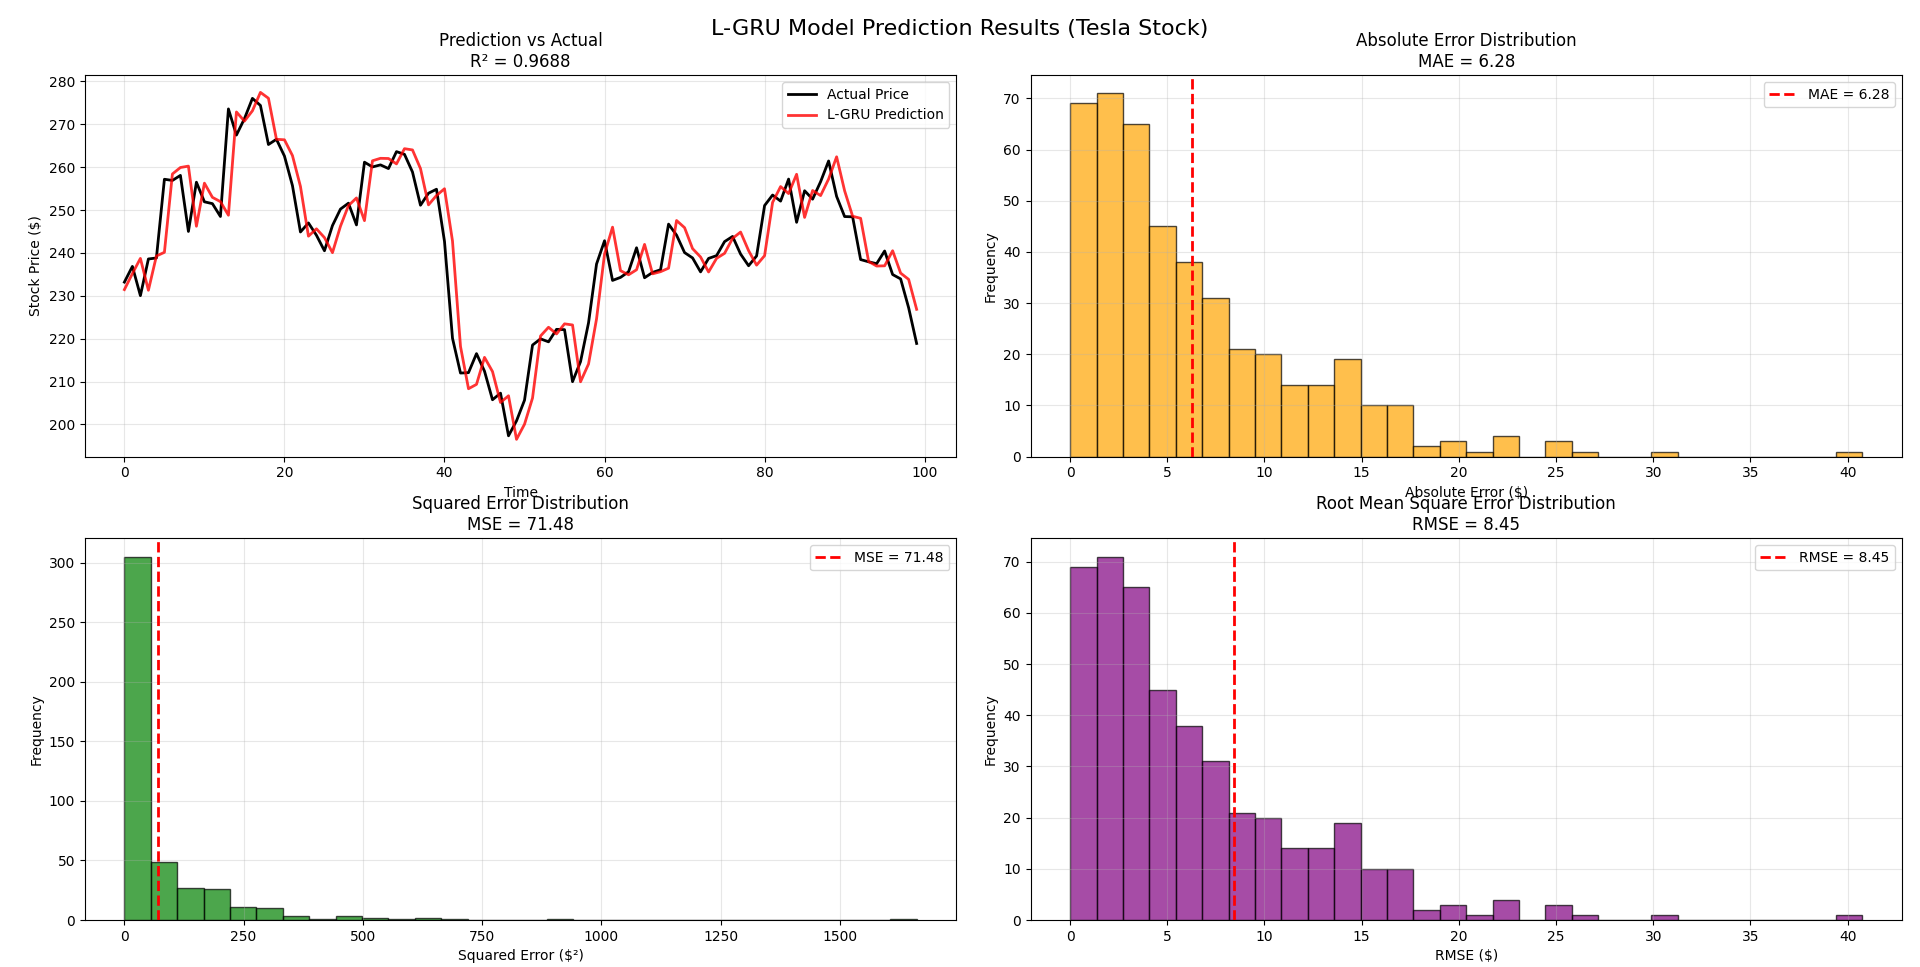
\includegraphics[width=\textwidth]{Figure/Figure_1.png}
        \caption{Execution Results of the L‑GRU Model}
        \label{fig:execution}
    \end{figure*}

    The empirical results unequivocally demonstrate the superior performance of the proposed L-GRU model across all evaluation metrics. A detailed analysis reveals several key insights:
    \begin{itemize}
        \item \textbf{Overall Superiority:}
        The L-GRU model achieves an R² score of 0.9688, indicating that it can explain approximately 96.8\% of the variance in the TSLA stock price, a remarkably high value that signifies an excellent fit to the data. In contrast, the next best model, GRU, achieves an R² of 0.9352. Furthermore, L-GRU's error metrics are substantially lower than those of all baseline models. It reduces the MAE by approximately 35\% compared to the best baseline (GRU) and cuts the MSE by more than half (a 52\% reduction). This translates to a significantly lower RMSE of 8.43, implying that the typical prediction error of the L-GRU model is substantially smaller than that of its counterparts.
        \item \textbf{L-GRU vs. LSTM and GRU:}
        The comparison with its parent architectures is particularly illuminating. While the standard GRU outperforms the standard LSTM on this dataset, the L-GRU model surpasses both by a wide margin. This strongly supports our central hypothesis. The L-GRU's superiority over the GRU suggests that while the GRU's efficient gating mechanism is effective, its merging of the cell and hidden states constitutes a loss of information that is critical for modeling complex financial data. By reintroducing the dedicated cell state from LSTM, L-GRU preserves this vital long-term memory channel. Simultaneously, its outperformance of the LSTM suggests that the GRU-inspired unified update gate and relevance gate are not only more efficient but can also lead to more effective learning dynamics than the separate input/forget gates of the LSTM, especially when augmented with architectural refinements like Layer Normalization and peephole connections. The L-GRU thus successfully synthesizes the most potent elements of both architectures.
        \item \textbf{L-GRU vs. Transformer:}
        The Transformer model, despite its power in other domains, exhibited the weakest performance among the four models on this specific task. This outcome can be attributed to several factors. First, financial time series data possesses a strong, inherent sequential and temporal ordering that recurrent architectures are naturally designed to exploit. The Transformer's self-attention mechanism, which treats the sequence as a set of tokens, may lose some of this crucial inductive bias. Second, the quadratic complexity of self-attention can be a bottleneck, and for a univariate forecasting task, its ability to find complex global dependencies may be less critical than the path-dependent memory accumulation at which RNNs excel. The superior performance of L-GRU highlights that for this class of problems, a well-designed recurrent architecture can be more effective and efficient.
        \item \textbf{L-GRU vs. CNN-LSTM:}
        The CNN-LSTM model excels at identifying local patterns before modeling temporal sequences. However, the superior performance of L-GRU suggests that its refined internal gating mechanism and direct handling of the temporal sequence are more effective for this specific financial dataset than the hierarchical feature extraction approach of CNN-LSTM. The L-GRU's architecture appears better suited to capturing the endogenous dynamics of the time series without the need for a separate feature extraction layer.
        \item \textbf{L-GRU vs. LSTM-Transformer:}
        The LSTM-Transformer combines sequential modeling with a powerful attention mechanism. While theoretically robust, its performance relative to L-GRU suggests that the added complexity of the self-attention mechanism may not yield proportional benefits for this univariate forecasting task. The L-GRU, with its more streamlined and temporally focused architecture, achieves a more efficient and accurate representation of the data's underlying process. This highlights that for certain time series problems, a sophisticated recurrent structure can be more potent than a combination involving global attention.
    \end{itemize}
    In conclusion, the empirical evaluation confirms that the L-GRU model provides a significant advancement in predictive accuracy for stock price forecasting. Its carefully engineered hybrid architecture, which balances the memory fidelity of LSTM with the computational efficiency of GRU and is enhanced with modern neural network techniques, establishes a new and powerful benchmark for financial time series analysis.
    \end{enumerate}
\section{Conclusions}\label{sec:conclusion}
The formidable challenge of accurately forecasting stock market prices, a domain characterized by inherent non-stationarity, high volatility, and complex temporal dependencies, has perpetually driven the quest for more sophisticated and robust predictive models. This research was motivated by the identified architectural trade-offs between the two leading recurrent neural network paradigms: the high-fidelity memory control of Long Short-Term Memory (LSTM) networks and the computational efficiency of Gated Recurrent Units (GRUs). We hypothesized that a novel hybrid architecture could be engineered to synergistically combine the strengths of both, thereby achieving a superior balance of predictive accuracy and operational efficiency.

This paper introduced the L-GRU, a novel hybrid recurrent neural network cell designed explicitly for financial time series forecasting. The core contribution of this work is the principled synthesis of the most potent components from both LSTM and GRU architectures. The L-GRU retains the dedicated, unadulterated cell state of the LSTM, which is critical for preserving the integrity of long-term dependencies, while operating this memory mechanism with a more efficient, GRU-inspired gating structure. This foundational design was further enhanced with advanced techniques, including decoupled weight matrices for specialized information processing, peephole connections for improved contextual awareness within the cell, and Layer Normalization for enhanced training stability.

The empirical evaluation, conducted on a challenging and volatile dataset of Tesla (TSLA) stock prices, provides compelling evidence supporting our hypothesis. The L-GRU model demonstrated unequivocally superior performance, outperforming established baseline models—LSTM, GRU, and the attention-based Transformer—across a comprehensive suite of evaluation metrics. Notably, the L-GRU achieved a Coefficient of Determination (R²) of 0.9688 and significantly reduced the Root Mean Squared Error (RMSE) to 8.45, a substantial improvement over the next best-performing model. These results validate the architectural choices made in the L-GRU design and establish it as a new, powerful benchmark for the task. The findings suggest that for this class of problem, a meticulously designed recurrent architecture that optimizes the interplay between memory preservation and gating efficiency can be more effective than both its parent architectures and alternative paradigms like the Transformer.

The implications of this research are twofold. From a theoretical standpoint, the success of the L-GRU model underscores the significant potential of hybrid deep learning architectures. It demonstrates that innovation can arise not only from entirely new paradigms but also from the intelligent and synergistic recombination of existing, proven concepts. Our work provides a successful blueprint for how to balance competing architectural desiderata—in this case, memory fidelity versus computational parsimony. From a practical perspective, the L-GRU model offers a tangible tool for financial practitioners, including investors, portfolio managers, and quantitative analysts. Its enhanced predictive accuracy can translate into more informed and data-driven decision-making, potentially leading to more effective trading strategies, improved risk management protocols, and a deeper quantitative understanding of market dynamics.

Despite the promising results, this study is subject to certain limitations which, in turn, open up avenues for future research. First, our analysis was confined to a univariate forecasting framework, utilizing only historical closing prices. The complex dynamics of the stock market are driven by a multitude of variables, including trading volume, technical indicators, macroeconomic data, and market sentiment. Second, the model's efficacy was demonstrated on a single financial instrument. While TSLA is a representative example of a high-volatility stock, the model's generalizability across different assets, market sectors, and economic conditions warrants further investigation. Third, like all deep learning models, the performance of L-GRU is contingent upon the selection of hyperparameters, and while a rigorous tuning process was followed, a more exhaustive search could potentially yield further performance gains.

Building upon this work, we propose several promising directions for future research. A natural next step is to extend the L-GRU architecture to a multivariate framework, enabling it to process a richer set of input features simultaneously. Another compelling avenue is the integration of the L-GRU model with Natural Language Processing (NLP) techniques to incorporate unstructured textual data, such as financial news, analyst reports, and social media sentiment, which are known to be significant drivers of market behavior. Furthermore, future work should focus on validating the L-GRU model's robustness and performance across a diverse portfolio of international stocks and other classes of financial assets, such as cryptocurrencies, commodities, and foreign exchange rates. Finally, further architectural explorations, such as the integration of attention mechanisms within the L-GRU cell or the development of adaptive gating mechanisms, could lead to even more powerful and sophisticated forecasting models.


% \section*{Acknowledgment}
% This research is funded by Eaut Asia University of Technology.

\vspace{12pt}
\bibliography{ref_all.bib}
\bibliographystyle{IEEEtran}
Article received on .....; accepted on ...... 
*Corresponding author is Nguyen Viet Hung. 

\end{document}
